% !TeX spellcheck = en_US
\section{Highspeed Digital Design}
\subsection{Time and distance}
Some facts:
\begin{itemize}
	\item Time on a 10\,mm long wire on FR4:  \qquad $t=71$\,ps
	\item Time of light from nose to the eye: \qquad $t=100$\,ps
	\item Transmission line is a low pass: 1\,dB/dek.
	\item Rise and fall time short as possible $\rightarrow$ hight frequency
\end{itemize}

\begin{table}[!h]
	\centering
	\begin{tabular}{|c|c|}
		\hline
		propagation delay &                                $\tau = \frac{\sqrt{\varepsilon}}{c}$ \quad $[\frac{s}{m}]$                                \\ \hline
		effective length  & $ l_{\text{eff}} = \frac{\text{time duration}}{\text{propagation delay}} = \frac{t}{\tau} \qquad t:$\,z.B. rise/fall-Time \\ \hline
		   Wire length    &                                       $l_{\text{wire}} > \frac{l_{\text{eff}}}{6}$                                        \\ \hline
	\end{tabular}
\end{table}

\begin{figure}[h]
	\centering
	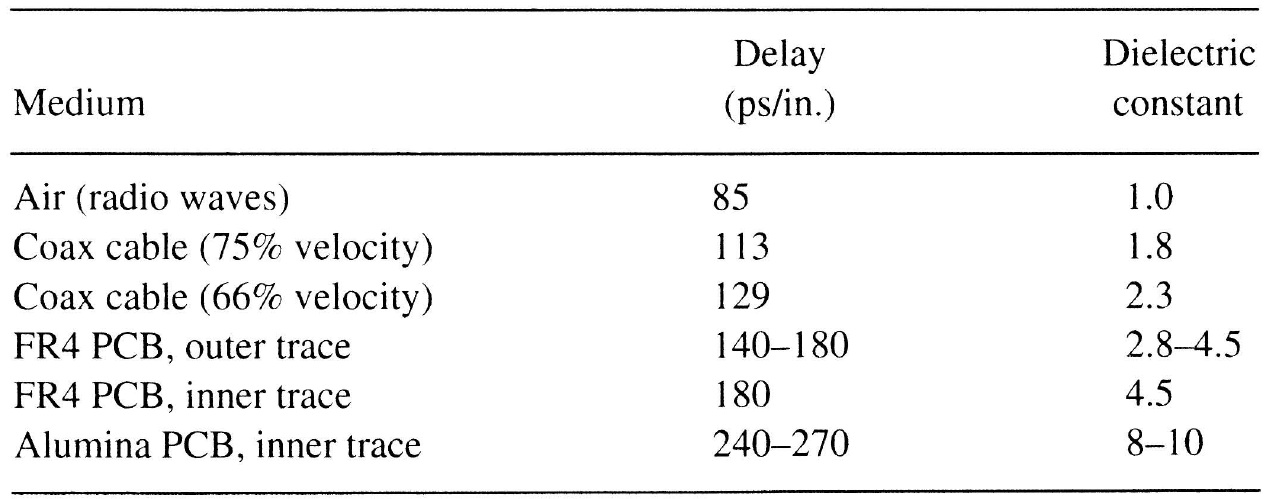
\includegraphics[width=0.4\textwidth]{images/High_Speed_Digital/propDelay.jpg}
	\caption{propagation delay}
\end{figure}

\subsection{Clock and clock free signaling}
\begin{table}[!h]
	\centering
	\begin{tabular}{|c|c|}
		\hline
		       \textbf{parallel signaling}         &              \textbf{serial signaling}              \\ \hline\hline
		          many bits in parallel            & only one serial line; all bits onbe after the other \\ \hline
		       lines for data must be sync         &  maximize clock speed, consider only one data line  \\ \hline
		$\Delta$ in line length reduces throughput &              no skew (dt. Bitversatz)               \\ \hline
		             lower throughput              &                  higher throughput                  \\ \hline
		            z.B: ISA,ATA,SCSI              &               z.B:  RS-232, USB, I2C                \\ \hline
	\end{tabular}
\end{table}

\subsubsection{Data rate}

\begin{description}
	\item [Bit rate:]\hfill \\
		 Number of transmitted bit per seconds \quad $[\frac{\text{bit}}{s}]$
	\item [Symbol rate:] \hfill \\
		 Number of transmitted symbols per seconds \quad $[\frac{\text{symbols}}{s} = \text{baud}]$
	\item [Channel capacity:] \hfill \\
		 Shannon-Theorem \\
		R : Information rate \quad $[\frac{\text{bit}}{s}]$\\
		C : Channel capacity \quad $[\frac{\text{bit}}{s}]$\\
		If $R<C$ then, exist a coding, which reduce the error rate by the receiving part close to zero.		
\end{description}

\begin{table}[!h]
	\centering
	\begin{tabular}{|c|c|}
		\hline
		AWGN channel & $C = B \cdot \log_2 \left( 1 + \frac{S}{N} \right)$ \\ \hline
	\end{tabular}
\end{table}

\subsubsection{Coding}
\begin{table}[!h]
	\centering
	\begin{tabular}{|c|l|c|}
		\hline
		\multicolumn{3}{|c|}{\textbf{No Coding}}                                                                                                                   \\ \hline
		       Data        & \multicolumn{2}{|c|}{No-return-to-zero-coding (NRZ)}                                                                                  \\
		                   & \multicolumn{2}{|c|}{1: Hight, 0: Low}                                                                                                \\
		      Clock        & \multicolumn{2}{|c|}{Return-to-one (RTO) or Return-to-zero (RTZ)}                                                                     \\ \hline\hline
		      
		\multicolumn{3}{|c|}{\textbf{Manchester}}                                                                                                                  \\ \hline
		        0          & high $\Rightarrow$ low transmission & \multirow{2}{*}{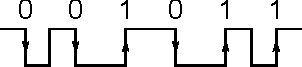
\includegraphics[width=0.25\textwidth]{images/High_Speed_Digital/Manchester-Code.pdf}} \\
		        1          & low $\Rightarrow$ high transmission &  \\ \hline
		\multicolumn{3}{|c|}{Clock recovery possible}                                                                                                              \\ \hline\hline
		
		\multicolumn{3}{|c|}{\textbf{CMI-Codieng (Code Mark Inversion)}}                                                                                           \\ \hline
		        0          & high $\Rightarrow$ low transmission & \multirow{3}{*}{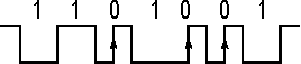
\includegraphics[width=0.25\textwidth]{images/High_Speed_Digital/CMI-Code.pdf}} \\
		\multirow{2}{*}{1} & low \quad if before high            &  \\
		                   & high \quad if before low            &  \\ \hline
		\multicolumn{3}{|c|}{Clock recovery possible}                                                                                                              \\ \hline\hline
		
		\multicolumn{3}{|c|}{\textbf{Redundancy-Coding}}                                                                                                           \\ \hline
		\multicolumn{3}{|c|}{Send more bits as necessary, for extra error detection and error correction}                                                          \\ \hline
		\multicolumn{3}{|c|}{example: Hamming-Coding}                                                                                                              \\ \hline\hline
		
		\multicolumn{3}{|c|}{\textbf{Differential-Signaling}}                                                                                                      \\ \hline
		\multicolumn{3}{|c|}{allows high speed by low signal voltage}                                                                                              \\ \hline
		\multicolumn{3}{|c|}{No ground line necessary}                                                                                                             \\ \hline
		\multicolumn{3}{|c|}{No common mode noise}                                                                                                                 \\ \hline
		\multicolumn{3}{|c|}{example: LVDT (Low-Voltage-Differential-Signaling), PCI-Express}                                                                      \\ \hline\hline
		
		\multicolumn{3}{|c|}{\textbf{Multi-Level-Code [Quadrature-Amplitude-Modulation (QAM)]}}                                                                    \\ \hline
		\multicolumn{3}{|c|}{Transmit of more then one bit per symbol \quad  $2^n$\,-QAM $\Rightarrow$ $n$ Bits}                                                   \\ \hline
		\multicolumn{3}{|c|}{Used in wireless communication}                                                                                                       \\ \hline

	\end{tabular}
\end{table}

\newpage
\subsubsection{Clock-driven and clock-less signaling}
\begin{table}[!h]
	\centering
	\begin{tabular}{|c|c|}
		\hline
		\textbf{Clock-Driven Signaling} &             \textbf{Clock-Less Signaling}              \\ \hline\hline
		Clock are separate transmitted  &         clock are contain in the data signals          \\ \hline
		                                & clock must be recovered / restore from the data signal \\
		                                &               Clock-Data-Recovery (CDR)                \\ \hline
		      examples: I2C, DDR2       &                    example: USB 3.0                    \\ \hline
	\end{tabular}
\end{table}

\subsubsection{Clock-Data-Recovery (CDR)}
\begin{description}
	\item [Goal:] \hfill \\
		 Extract the clock-signal form the data-signal
	\item [Method:] \hfill \\
		 A Phase-Locked-Loop (PLL) controls the phase and the frequency. The data-signal are the reference (Soll-Wert). The easiest phase detector (Diskiminator) is a D-Flip-Flop. Other complex phase detector are:
		\begin{itemize}
			\item Hogge Phase-Detector
			\item Alexander Phase-Detector
			\item Half-Rate Phase-Detector
			\item Quarter-Rate Phase-Detector
			\item N-th R Phase-Detector:\\
				If the date-rate is too high, so that the design of the VCO became to complex. In this case, the design complexity of the VCO can be reduced by divied the frequency to the factor $2^n$ and a $n$-th rate Phase-Detector are be used. 
		\end{itemize}
\end{description}
\begin{figure}[h]
	\centering
	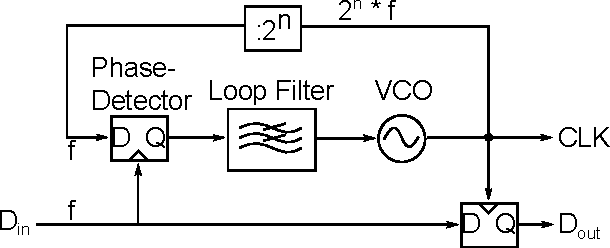
\includegraphics[width=0.5\textwidth]{images/High_Speed_Digital/PLL.pdf}
	\caption{propagation delay}
\end{figure}


\subsection{Timing Analysis}
\begin{description}
	\item[Goal:] \hfill \\
		To check whether the timing specifications are met. The timing analysis are used to check the component timing-specification so that they are respected (dt. eingehalten werden). To check that the system-coordination are works or correct (the component can problem-free communicate) , the timing-analysis can be used.
\end{description}

\newpage
\subsubsection{Static TA vs. Dynamic TA}
\begin{table}[!h]
	\centering
	\begin{tabular}{|c|c|}
		\hline
		         \textbf{Static TA (STA)}          &             \textbf{Dynamic TA (DTA)}             \\ \hline\hline
		calculates timing-path without simulations &                 timing simulation                 \\ \hline
		   always covers extremes  (worst case)    &         may fail to find the longest path         \\ \hline
		                                           & can simulate systems with different clock-regions \\ \hline
	\end{tabular}
\end{table}

\begin{description}
	\item[Note:] \hfill \\
		The Static TA (STA) is not able to cover interfaces between different clock regions!
\end{description}

\subsubsection{Static Tining Analysis}
\begin{multicols}{2}
    Consider four types of paths:
    \begin{enumerate}
        \item \textcolor{orange}{clock-to-clock}
        \item \textcolor{green}{input-to-clock}
        \item \textcolor{blue}{clock-to-output}
        \item \textcolor{red}{input-to-output}
    \end{enumerate}
    \vfill
    \columnbreak
    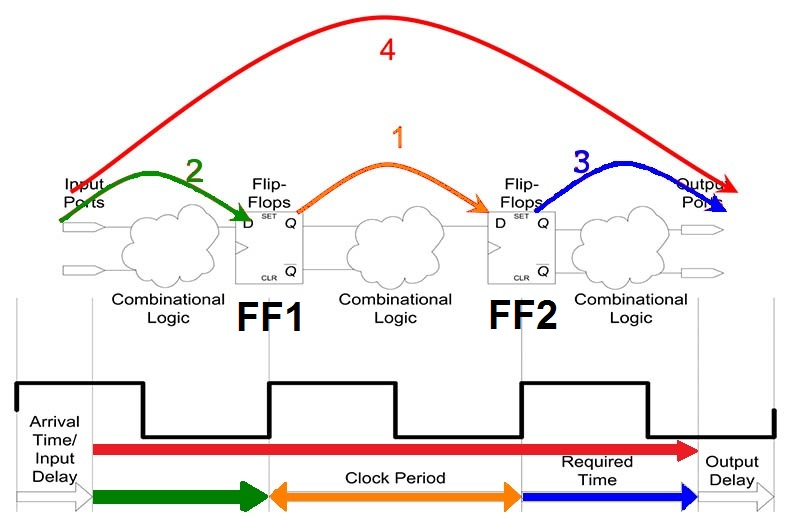
\includegraphics[width=0.7\linewidth]{images/High_Speed_Digital/HSDigital_TimingAnalysis.jpg}
    %TODO: draw nice picture in TikZ (hmm... das chani leider nonig ;) )
\end{multicols}

Consider: minimum / maximum delays, dependence on voltage, temperature, process, load, edge (rising/falling)

\begin{table}[!h]
	\centering
	\begin{tabular}{|l|c|}
		\hline
		\textcolor{orange}{1. clock-to-clock} & $t_{\text{path}} \leq T_{\text{CLK}} + t_{\text{CLK} \rightarrow \text{FF2}} - t_{\text{CLK} \rightarrow \text{FF1}}$ \\ \hline
		\textcolor{green}{2. input-to-clock}  &                           $t_{\text{path}} = t_{\text{comb-logik}} + t_{\text{setupFF1}} $                            \\
		                                      &        $t_{\text{path}} \leq T_{\text{CLK}} + t_{\text{CLK} \rightarrow \text{FF1}} - t_{\text{input-delay}}$         \\ \hline
		\textcolor{blue}{3. clock-to-output}  &                              $t_{\text{path}} = t_{\text{FF2}} + t_{\text{comb-logik}}$                               \\
		                                      &        $t_{\text{path}} \leq T_{\text{CLK}} - t_{\text{CLK} \rightarrow \text{FF2}} - t_{\text{output-delay}}$        \\ \hline
		\textcolor{red}{4. input-to-output}   &                                      $t_{\text{path}} = t_{\text{comb-logik}} $                                       \\
		                                      &               $t_{\text{path}} \leq T_{\text{CLK}} - t_{\text{input-delay}} - t_{\text{output-delay}} $               \\ \hline
		multi-clock-cycle-path                &                               Combinational logic needs longer then the one clock-cycle                               \\ \hline
		false path                            &                            path exist physical, but it will not be used (no data transfer)                            \\ \hline
	\end{tabular}
\end{table}

\paragraph{Clock-to-clock}The maximal path consists of 
\begin{itemize}
    \item $t_{PCQ}$: max. clock-to-output delay of flip-flop
    \item $t_{NET}$: max. data path between flip-flops
    \item $t_{SETUP}$: max. data setup time to clock of second flip-flop 
    \item $t_{CLK(1)}$: min. delay of the clock signal of the first flip-flop
    \item $t_{CLK(2)}$: max. delay of the clock signal of the second flip-flop
\end{itemize}

Static timing analysis on base of a schematic assumes standard net lengths (a 2-pin net is assumed to be shorter than a 3-pin net, etc.).

\begin{multicols}{2}
    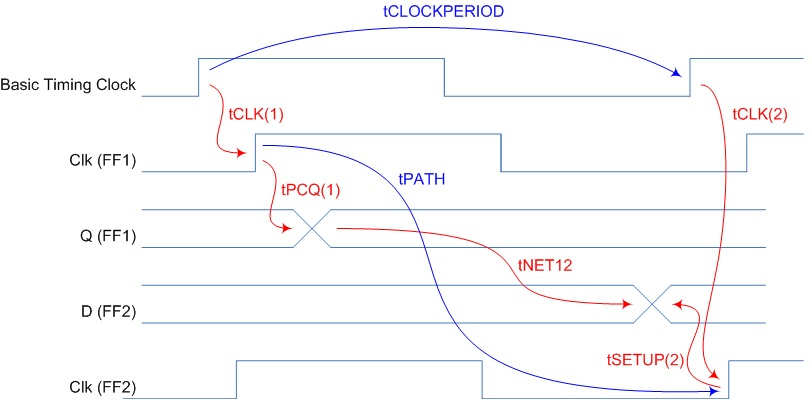
\includegraphics[width=0.9\linewidth, height=0.5\linewidth]{images/High_Speed_Digital/clock-to-clock.jpg} \\
    \vfill
    \columnbreak
    The maximal path must be shorter than the clock period (plus the delay from the clock source to the second flip-flop, minus the delay from the clock source to the first flip-flop)
\end{multicols}

%TODO: maybe add example?

\subsubsection{Gate delays and wire delays}
\paragraph{Delays}There exist two types of delay: \emph{gate} delays and \emph{wire} delays. \\
\begin{table}[htbp]
    \centering
    \begin{tabularx}{0.9\linewidth}{XX}
        Gate delays & Wire delays \\ \toprule
        \begin{circuitikz} \draw (0,0) node[not port] {} (1,0); \end{circuitikz}
        & \tikz[scale=0.5]{\draw (0,0)--(1,0)--(1,1)--(2,1) (1,0)--(1,-1)--(2,-1)--(2,-0.5)--(3,-0.5) (2,-1)--(2,-1.5)--(3,-1.5); \draw[fill=black] (1,0) circle (0.1) (2,-1) circle (0.1);}  \\
        through transistors, semiconductors & through wires \\
        dependent on:  \newline
        - temperature (higher $\to$ higher delays)\newline
        - voltage (higher $\to$ lower delays)\newline
        - load (higher $\to$ higher delays)\newline
        - technology, \dots
        & dependent on:\newline
        - length of wire (higher $\to$ higher delays)\newline
        - resistance of wire (higher $\to$ higher delays)\newline
        - temperature (higher $\to$ higher delays)\newline
        - low dependency on temperature \newline
        - capacitance, inductance, \dots \newline
        - low dependency on temperature \newline
        \textbf{influences are not significant!!!}\\
        \bottomrule
    \end{tabularx}
\end{table}

\paragraph{Conditions}Commercial: BCC (Best case Commercial) is the fastest, WCC (Worst Case Commercial) is the slowest case. Other conditions: Industrial (BCI, WCI), Military (BCM, WCM) \\

\paragraph{Multi clock cycle path}A combinatorial which takes more time than one clock cycle. 
Problem: you do not always know, when the signal arrives at the output. 
Solution: e.g. define \emph{clock enable} signal and latch only e.g. every fourth input to the logic part and the output.

\paragraph{False path}A path which physically exists, but is never used, e.g.
\begin{itemize}
    \item Two MUX in series, not all paths are logically possible
    \item False path to define a relation between two asynchronous clocks
    \item Test logic, which would not run at full speed and is not optimized for speed.
\end{itemize}


\subsubsection{Dynamic Timing Analysis}
\paragraph{Cycle based simulation}
Events only happen at clock edges, thus no delays are considered.
Cycle based simulation is purely \emph{functional}.
\paragraph{Unit delay simulation}
Assumes a standard delay, which leads to a simple model. Not very relevant.
\paragraph{Prelayout timing simulation}
Uses propagation times from data sheets and standard values.
\begin{itemize}
	\item delays for Gate  $\Rightarrow$ datasheet
	\item delays from wire $\Rightarrow$ standard values
\end{itemize}
\paragraph{Postlayout timing simulation}
Uses actual wire geometries, including parasitics.
By far the slowest, but the only really accurate timing simulation.

\subsubsection{Clock Distribution Schemes}

\paragraph{Common-clock distribution timing}
\begin{itemize}
	\item Common (third-party) clock used by driver and receiver.
	\item  OK for up to \SI{200}{\mega\hertz}.
\end{itemize} 

\paragraph{Source synchronous clocking}
\begin{itemize}
	\item Driver sends clock and data
	\item Driver delays data slightly.
\end{itemize}

\paragraph{Incident synchronous}
\begin{itemize}
	\item Driver send data and clock at the same time
	\item Receiver delayed the data signal.
\end{itemize}


\paragraph{Embedded clocking}
\begin{itemize}
	\item Clock is embedded in data (e.g. Manchester coding).
	\item Data and clock have the same delay
	\item Receiver recover the clock from the data-signal, and control the delay itself.
\end{itemize}

\subsection{Clock-Signal}
\begin{tabbing}
	\hspace{10mm} \= \hspace{5mm} \= \\
	\textbf{Time-Slack}	 \hfill \\
						\>$\bullet$ \> reserve of the path-time $\geq$ 0 \\
						\>$\bullet$ \>available path-time minus used path-time 
\end{tabbing}
	
\begin{multicols}{2}
	\begin{tabbing}
	\hspace{10mm} \= \hspace{5mm} \= \\
	\textbf{Jitter}\hfill \\
						\>$\bullet$ \> fast variation or fluctuations of the clock frequency \\
						\>$\bullet$ \> different between real and ideal clock edge \\
						\>$\bullet$ \> Superposition of noise from other signals \\
		 				\> \>(example: Thermal-, Amplifier-, Power-supply-, PLL-control noise)
	\end{tabbing}
	\vfill
	\columnbreak
	\hspace{40mm}
	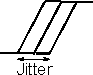
\includegraphics[width=0.3\linewidth]{images/High_Speed_Digital/Jitter.pdf}
\end{multicols}
	
\begin{multicols}{2}
	\begin{tabbing}
		\hspace{10mm} \= \hspace{5mm} \= \\
		\textbf{Skew} \hfill \\
						\>$\bullet$ \> different between fastest and lowest arrival time of\\
						\> \> the clock-signal at different receivers.\\
						\>$\bullet$ \> caused by different lengths of lines.
	\end{tabbing}
	\vfill
	\columnbreak
	\hspace{40mm}
	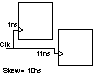
\includegraphics[width=0.35\linewidth]{images/High_Speed_Digital/Skew.pdf}
\end{multicols}

\subsubsection{Clock-signal properties}
The clock-signal should be have the following properties

\begin{description}
	\item[Monoton], to prohibit double clocks. \\
		$\Rightarrow$ Oscillation will be produced by reflection on the load or source. \\
		$\Rightarrow$ Critical are reflection on the load $\rightarrow$ double clocks
		
	\item[Fast], to reduce the uncertainty (dt. Unsicherheit) of the clock-edge position. \\
		$\Rightarrow$ ideal rectangle \\
		$\Rightarrow$ but, faster the edge, then more likely to Ringing ($\rightarrow$ double clocks) 
	
	\item[High fan out driver], to increase the clock-edge. \\
		$\Rightarrow$ Clock-driver are the most loaded signal
		
	\item[Low Jitter], to increase the time-sack on a single receiver. \\
	    $\Rightarrow$ receiver can be a Flip Flop. \\
		$\Rightarrow$ \textbf{Clock-Jitter reduce the clock-periode}
		
	\item[Low Skew], to increase the time-sack on more then one single receiver. \\
		$\Rightarrow$ \textbf{Clock-Skew reduce the clock-periode}
\end{description}

\textbf{\textcolor{red}{A reduction of the Clock-Jitter, increments the Clock-Skew}}
\begin{equation*}
	\boxed{\text{Jitter} \sim \frac{1}{\text{Skew}}}
\end{equation*} 

\subsubsection{Clock-Skew}
\begin{description}
	\item[The path-delay must be smaller than the clock-period] \hfill \\
		\fcolorbox{orange}{orange}{$t_{\text{path}} < T_{\text{CLK}} + t_{\text{skew}}$}
		\begin{multicols}{2}
			if $t_{\text{path}} > T_{\text{CLK}} + t_{\text{skew}}$: \\
			$\bullet$ increase clock-period $T_{\text{CLK}}$ $\Rightarrow$ $f_{\text{CLK}}$ will be smaller\\
			$\bullet$ increase delay to FF2 ($t_{\text{skew}}$ will be bigger).\\
			$\bullet$ use faster flip-flop for FF1 (faster technology.)\\
			$\bullet$ manually clock roting from first to the last flip-flop.
			\vfill
			\columnbreak
			\hspace{5mm}
			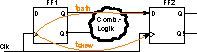
\includegraphics[width=1\linewidth]{images/High_Speed_Digital/Clock-Skew.pdf}
		\end{multicols}
		
	\item[clock-skew must be smaller than the shortest path-delay] \hfill \\
		\fcolorbox{orange}{orange}{$t_{\text{skew}} < \min \left( {t_{\text{path}}} \right)$} \\ \\
		otherwise goes the the input of FF1 ($D_{\text{FF1}}$) a clock-cycle after the output of FF2 ($Q_{\text{FF2}}$)\\
		$\bullet$ problem gets worse at faster technology $\Rightarrow$ switch to slower technology\\
		$\bullet$ reduce clock-delay of FF2 $\Rightarrow$ slower $t_{\text{skew}}$ \\
		$\bullet$ manually clock roting from first to the last flip-flop. \\
		$\bullet$ use slower flip-flop for FF1 \\
		$\bullet$ insert a buffer between FF1 and FF2	
\end{description}

\subsubsection{Clock-Jitter}
\begin{itemize}
	\item PLL clock-generator produce Clock-Jitter
	\item Clock-Jitter spread the clock-frequency-spectrum
	\begin{itemize}
		\item $\Rightarrow$  Clock-Jitter can be improve by filtering
		\item Clock-Divider: Jitter $\approx$ 200\,fs $\ldots$ 250\,fs
		\item LC-Bandpass-Filter: Jitter $\approx$ 100\,fs
		\item Crystal-Filter: Jitter $\approx$ 50\,fs
	\end{itemize}
	\item Clock-Jitter are consciously (dt. bewusst, absichtlich) add, to reduce power-peaks
	\item In Analog-Digital-Converter, Clock-Jitter lead to Jitter-Noise (Sample-Time-Noise)
\end{itemize}

\begin{equation*}
	\boxed{\text{SNR} = -20 \log_{10} \left( 2 \pi f T_j \right) \qquad T_j: \text{RMS of the Jitter aperture}}
\end{equation*}

\begin{figure}[h]
	\centering
	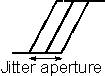
\includegraphics[width=0.2\textwidth]{images/High_Speed_Digital/Jitter-Aperture.pdf}
	\caption{Jitter-Aperture}
\end{figure}
\subsection{Power Consumption}
\subsubsection{Where is the Energy dissipated}
\begin{description}
	\item[Load and discharge of the capacity (at each clock-edge)] \hfill \\
		\fcolorbox{orange}{orange}{$E_{\text{CK}} = \frac{1}{2} C_k \cdot U_{\text{DD}}^2$}   \quad $C_k \approx C_{\text{gate}} + C_{\text{wire}}$; \quad $E_{\text{CK}} \sim \text{swich-frequency}$ \quad $E_{\text{CR}} \sim C_k$
		
	\item[Transistor switching ] \hfill \\
		\fcolorbox{orange}{orange}{$E_{\text{CR}} = \frac{\beta}{12} \left( U_{\text{DD}} - 2\cdot U_{text{th}}\right)^3 \cdot t_{\text{rak}}$}   \quad $\beta$: gain; \quad $t_{\text{rak}}$: ramp-time;  \quad $U_{text{th}}$: threshold-voltage; \\\\ \quad $E_{\text{CK}} \sim \text{swich-frequency}$ \quad $E_{\text{CK}} \sim$ slowness of the slope

	\item[Static current through resistor] \hfill \\
		\fcolorbox{orange}{orange}{$P_{\text{RR}} = \frac{U_{\text{DD}}^2}{R}$}   \quad $P_{\text{RR}} \sim U_{\text{DD}}^2$; \quad $P_{\text{RR}} \sim \frac{1}{R} = G$\\\\
		example: Pull-Up, Pull-Down Resistor, amplifier $\ldots$
		
	\item[Leakage current] \hfill \\
		$\bullet$ current increase with rising temperature (self-reinforcing, (dt. selbst verstärkend)) \\
		$\bullet$ frequency independent
\end{description}

\subsubsection{Why must be reduce Power Consumption}
\begin{tabbing}
	\hspace{10mm} \= \hspace{5mm} \= \\
	\textbf{General trend}	 \hfill \\
						\>$\bullet$ \>increase life time of the battery \\
						\>$\bullet$ \>smaller and lighter devices \\
							     \> \>$\rightarrow$ smaller batteries \\
							     \> \>$\rightarrow$ smaller cooling system \\
						\>$\bullet$ \>use new energy sources 
\end{tabbing}

\begin{tabbing}
	\hspace{10mm} \= \hspace{5mm} \= \\
	\textbf{increase life time of the electrical component}	 \hfill \\
						\>$\bullet$ \>heat reduce the life time \\
						\>$\bullet$ \>if less hot, then less cooling necessary
\end{tabbing}

\begin{tabbing}
	\hspace{10mm} \= \hspace{5mm} \= \hspace{30mm} \=\\
	\textbf{Temperature limit of the electronic component}	 \hfill \\
						\>$\bullet$ \>the component works correctly only in a definition temperature range \\
						\>$\bullet$ \>if less hot, then less cooling necessary \\
							     \> \>$\rightarrow$ Commercial: \> $0^\circ\text{C}$ $\ldots$ $70^\circ\text{C}$ \\
							     \> \>$\rightarrow$ Industrial: \> $-40^\circ\text{C}$ $\ldots$ $80^\circ\text{C}$\\
							     \> \>$\rightarrow$ Military:   \> $-55^\circ\text{C}$ $\ldots$ $125^\circ\text{C}$ \\
\end{tabbing}

\begin{tabbing}
	\hspace{10mm} \= \hspace{5mm} \= \\
	\textbf{Popcorn-Effect in poor storage}	 \hfill \\
						\>$\bullet$ \>Moisture inside plastic package causes explosion of package \\
						\>$\bullet$ \>No problem with ceramic packages (but ceramic packages are much more expensive!)
\end{tabbing}

\begin{tabbing}
	\hspace{10mm} \= \hspace{5mm} \= \\
	\textbf{Temperature density on PCB}	 \hfill \\
						\>$\bullet$ \>Different component temperature $\rightarrow$ deformation of the PCB \\
						\>$\bullet$ \>heating of the neighbor devices
\end{tabbing}
	
	
\newpage
\subsubsection{Current consumption calculation}
The current consumption consist off:
\begin{description}
	\item[Static current consumption (leaked current)] \hfill \\
		\fcolorbox{orange}{orange}{$P_S = \sum\limits_{i=1}^{n} I_{\text{leak}} \cdot U_{\text{supply}}$ \quad if $n=1$ $\Rightarrow$ $P_S = U_{\text{CC}} \cdot I_{\text{CC}} $ }  
		
	\item[Dynamic current consumption] \hfill \\
		\begin{description}
			\item[$\bullet$ Transient power (Gate-Switching)] \hfill \\
				\fcolorbox{orange}{orange}{$P_T = C_{\text{pd}} \cdot U_{\text{CC}}^2 \cdot f_{\text{in}} \cdot N_{\text{SW}}$} 
				%TODO MSP430 Beispiel hinzufügen
				
			\item[$\bullet$ Capacity-Load-Power (Output-Switching)] \hfill \\
				\fcolorbox{orange}{orange}{$P_L = \sum\limits_{i=1}^{N_{\text{SW}}} C_{\text{L}_i} \cdot f_{\text{out}_i} \cdot U_{\text{CC}}^2 $} 
		\end{description}	
	\item[Total current consumption] \hfill \\
		\fcolorbox{orange}{orange}{$P_{\text{TOT}} = P_S + P_T + P_L$} 
		\begin{tabbing}
			\hspace{10mm} 			\= \hspace{5mm} \= \\
				$U_{\text{CC}}$: 	\>Supply voltage \\
				$U_{\text{CC}}$: 	\>Supply voltage \\
				$I_{\text{CC}}$: 	\>Leaked current (dt. Kriechstrom) $\Rightarrow$ from datasheet \\
				$C_{\text{pd}}$: 	\>Power Dissipation Capacity $\Rightarrow$ from datasheet  \\
				$C_{\text{L}}$:  	\>External Load Capacity ($C_{\text{wire}} + C_{\text{input}}$)  \\
				$f_{\text{in}}$: 	\>input frequency (Clock or Data)  \\
				$f_{\text{out}}$: 	\>output signal frequency (Data) \\
				$N_{\text{SW}}$:	\> Number of (output) bits switching
		\end{tabbing}
 
\end{description}


\subsubsection{How to reduce Power Consumption}
\begin{tabbing}
	\hspace{10mm} \= \hspace{5mm} \= \\
						\>$\bullet$ \>reduce power-supply-voltage \\
						\>$\bullet$ \>chose low-power technology \\
						\>$\bullet$ \>use sleep and power-save modus \\
						\>$\bullet$ \>reduce operation frequency \\
						\>$\bullet$ \>reduce calculation effort (dt. Aufwand)\\
						\>$\bullet$ \>reduce chip-to-chip communication or chose a other interface type (for example: LVDT)  \\
						\>$\bullet$ \>optimize system architecture, for example: use internal memory \\
						\>$\bullet$ \>Latch based design. Replace flip-flop with Latches (Latch = half flip-flop) \\
						\>$\bullet$ \>Clock-Gating: Use different clock-region $\Rightarrow$ Every region have the clock that it necessary. \\
						\>$\bullet$ \>Power-Gating: Power off the region, which are not used. \\				
\end{tabbing}
